\documentclass[a2paper, 12pt]{article}
\usepackage[font={huge, bf}]{caption}
\usepackage{fontspec}
\setmainfont{Arial}
\usepackage{subcaption}
\usepackage{graphicx}
\usepackage{tikz}
\usepackage{tikzsymbols}
\usetikzlibrary{calc,patterns,shapes.geometric}
\usepackage{float}
\usepackage{pdflscape}
\usepackage{geometry}
\geometry{landscape, margin=2cm}
\captionsetup[subfigure]{justification=justified,singlelinecheck=false}
\pagestyle{empty}

\def\centerarc[#1](#2)(#3:#4:#5){\draw[#1] ($(#2)+({#5*cos(#3)},{#5*sin(#3)})$) arc (#3:#4:#5);}

\begin{document}
	\vspace*{\fill}
	\begin{figure}[!htbp]
		\centering
		\begin{subfigure}[b]{0.48\textwidth}
			\caption{Figure 1}
			\centering
			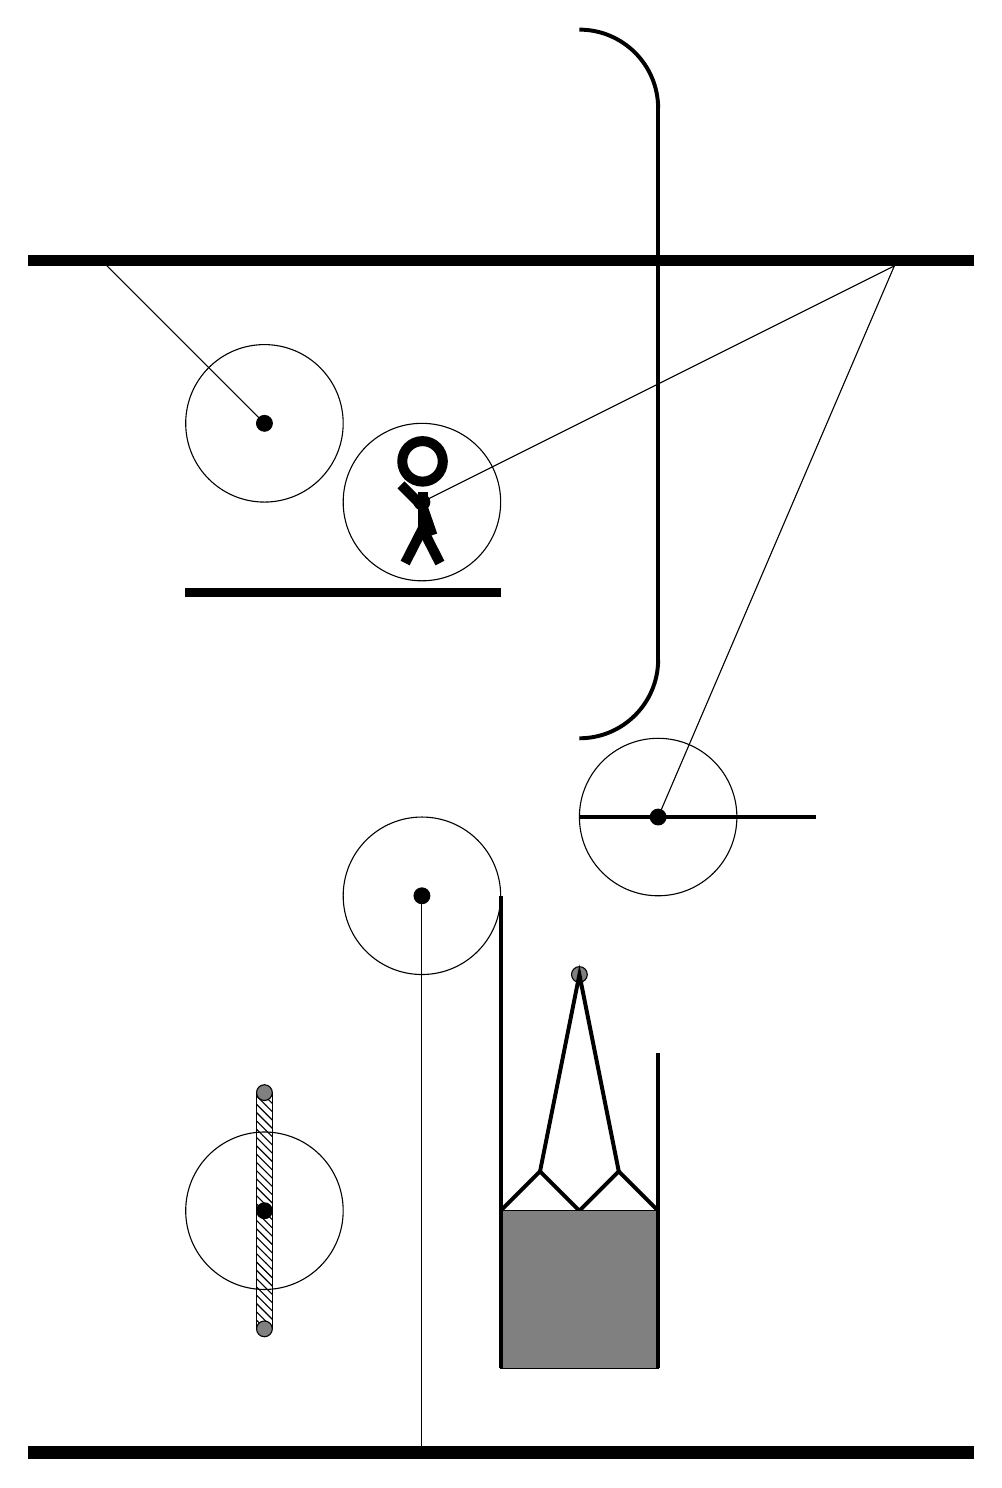
\begin{tikzpicture}
				\draw[fill=black] (-6, 12) rectangle (6, 12.125);
				
				\draw (-1,9) circle (1);
				\draw[fill=black] (-1,9) circle (0.1);
				\draw (5,12.0) -- (-1,9);
				
				\draw (-1,4) circle (1);
				\draw[fill=black] (-1,4) circle (0.1);
				\draw (-1,-3.15) -- (-1,4);
				
				\draw (-3,0) circle (1);
				\draw[fill=black] (-3,0) circle (0.1);
				\draw[pattern=north west lines, pattern color=black] (-3.1,1.5) rectangle (-2.9,-1.5);
				\draw[fill=black!50] (-3,1.5) circle (0.1);
				\draw[fill=black!50] (-3,-1.5) circle (0.1);
				
				\draw (-3,10) circle (1);
				\draw[fill=black] (-3,10) circle (0.1);
				\draw (-5,12.0) -- (-3,10);
				
				\draw (2,5) circle (1);
				\draw[fill=black] (2,5) circle (0.1);
				\draw (5,12.0) -- (2,5);
				
				\draw[fill=black!50] (1,3) circle (0.1);
				\draw[line width=0.5mm](0.5,0.5) -- (1,3) --  (1.5,0.5);
				\draw[line width=0.5mm](0,0) --  (0.5,0.5) -- (1,0) -- (1.5,0.5) -- (2,0);
				\draw[fill=black!50] (0, 0) rectangle (2, -2);
				
				\draw[line width = 0.5mm] (1,6) arc (270:360:1);
				\draw[line width = 0.5mm] (2,7) -- (2,14);
				\draw[line width = 0.5mm] (2,14) arc (0:90:1);
				\draw[line width = 0.5mm] (1,5) -- (4,5);
				\centerarc[line width = 0.5mm](1,4)(90:180:1);
				\draw[line width = 0.5mm] (0,4) -- (0,-2);
				\centerarc[line width = 0.5mm](1,-2)(180:360:1);
				\draw[line width = 0.5mm] (2,-2) -- (2,2);
				\centerarc[line width = 0.5mm](3,2)(0:180:1);
				
				\node at (-1, 9) {\scriptsize \Strichmaxerl[10][109][135]};
				\draw[fill=black] (-4, 7.9) rectangle (0, 7.8);
				
				\draw[fill=black] (-6, -3) rectangle (6, -3.15);
			\end{tikzpicture}
		\end{subfigure}
		\hfill
		\begin{subfigure}[b]{0.48\textwidth}
			\caption{Figure 2}
			\centering
			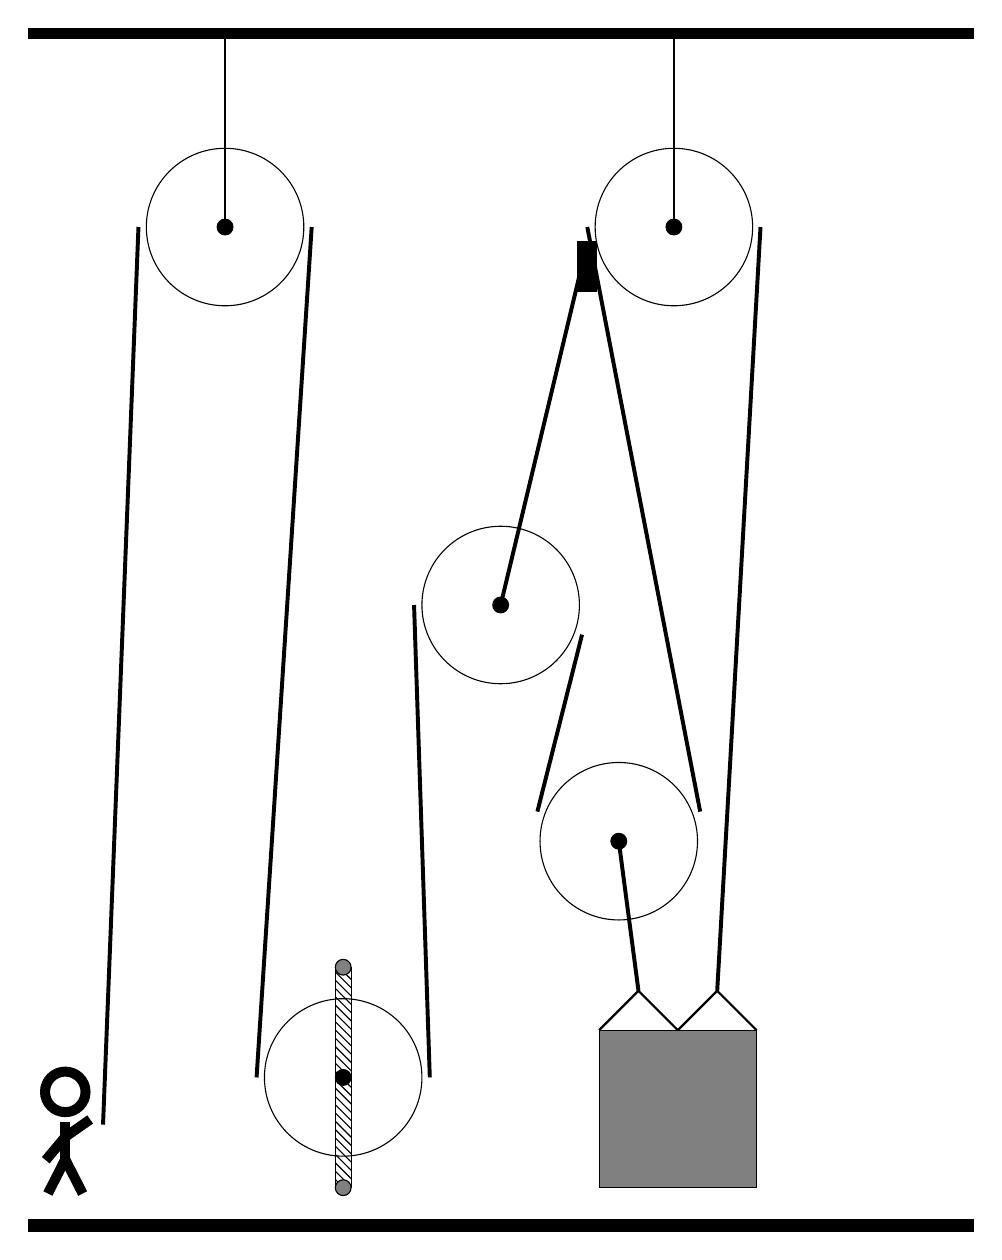
\begin{tikzpicture}
				\draw[fill=black] (-6, 12) rectangle (6, 12.125);
				
				\draw (0, 4.8) circle (1);
				\draw[fill=black] (0, 4.8) circle (0.1);
				
				\draw (1.5, 1.8) circle (1);
				\draw[fill=black] (1.5, 1.8) circle (0.1);
				
				\draw (2.2, 9.6) circle (1);
				\draw[fill=black] (2.2, 9.6) circle (0.1);
				\draw[thick] (2.2, 9.6) -- (2.2, 12);
				
				\draw (-3.5, 9.6) circle (1);
				\draw[fill=black] (-3.5, 9.6) circle (0.1);
				\draw[thick] (-3.5, 9.6) -- (-3.5, 12);
				
				\draw (-2, -1.2) circle (1);
				\draw[fill=black] (-2, -1.2) circle (0.1);
				\draw[pattern=north west lines, pattern color=black] (-2.1, 0.2) rectangle (-1.9, -2.6);
				\draw[fill=black!50] (-2, 0.2) circle (0.1);
				\draw[fill=black!50] (-2, -2.6) circle (0.1);
				
				\draw[thick]  (1.25, -0.6) -- (1.75, -0.1) -- (2.25, -0.6) -- (2.75, -0.1) -- (3.25, -0.6);
				\draw[fill=black!50] (1.25, -0.6) rectangle (3.25, -2.6);
				\draw[line width=0.5mm] (-5.05, -1.8) -- (-4.6, 9.6);
				\centerarc[line width=0.5mm](-3.5, 9.6)(0:180:1.1);
				\draw[line width=0.5mm] (-2.4, 9.6) -- (-3.1, -1.2);
				\centerarc[line width=0.5mm](-2, -1.2)(180:360:1.1);
				\draw[line width=0.5mm] (-0.9, -1.2) -- (-1.1, 4.8);
				\draw[line width=0.5mm] (0, 4.8) -- (1.1, 9.4);
				\draw[line width=0.5mm, fill=black](1.0, 8.8) rectangle (1.2, 9.4);
				\centerarc[line width=0.5mm](0, 4.8)(-20:180:1.1);
				\draw[line width=0.5mm] (1.0337, 4.4238) -- (0.4663, 2.1762);
				
				\centerarc[line width=0.5mm](1.5, 1.8)(160:380:1.1);
				\draw[line width=0.5mm] (2.5337, 2.1762) -- (1.1, 9.6);
				\draw[line width=0.5mm](1.5, 1.8) -- (1.75, -0.1);
				\centerarc[line width=0.5mm](2.2, 9.6)(0:180:1.1);
				\draw[line width=0.5mm] (3.3, 9.6) -- (2.75, -0.1);
				
				\node at (-5.5, -1.9) {\scriptsize \Strichmaxerl[10][50][35]};
				
				\draw[fill=black] (-6, -3) rectangle (6, -3.15);
			\end{tikzpicture}
		\end{subfigure}
	\end{figure}
		\vspace*{\fill}
\end{document}